\documentclass{standalone}

\usepackage[euler-digits]{eulervm}

\usepackage{tikz}
\tikzset{every node/.style={shape=circle,draw=none,minimum size=2.5mm,inner sep=0pt}}
%\tikzset{every node/.style={shape=circle,draw,minimum size=5mm,inner sep=0pt}}

\begin{document}
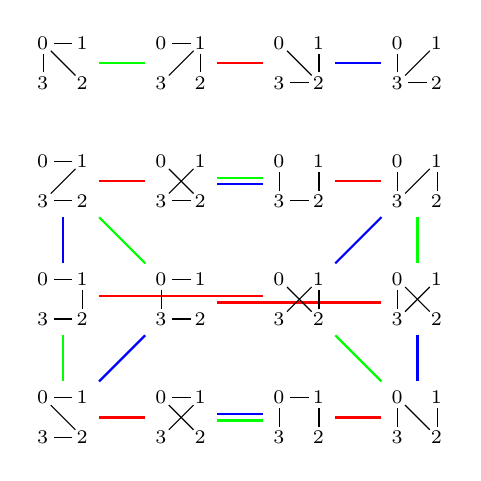
\begin{tikzpicture}[scale=0.5]

\tikzstyle{c}=[shape=rectangle,red,minimum size=9mm,opacity=0]
%\tikzstyle{c}=[red, inner sep=3mm,opacity=0]
%tikzstyle{c}=[red, inner sep=3mm]
\node[c] (A) at (0.5,9.5) {$A$};
\node[c] (B) at (3.5,9.5) {$B$};
\node[c] (C) at (6.5,9.5) {$C$};
\node[c] (D) at (9.5,9.5) {$D$};

\node[c] (4) at (0.5,6.5) {$4$};
\node[c] (5) at (3.5,6.5) {$5$};
\node[c] (3) at (6.5,6.5) {$3$};
\node[c] (6) at (9.5,6.5) {$6$};

\node[c] (1) at (0.5,3.5) {$1$};
\node[c] (12) at (3.5,3.5) {$12$};
\node[c] (2) at (6.5,3.5) {$2$};
\node[c] (11) at (9.5,3.5) {$11$};

\node[c] (9) at (0.5,0.5) {$9$};
\node[c] (8) at (3.5,0.5) {$8$};
\node[c] (10) at (6.5,0.5) {$10$};
\node[c] (7) at (9.5,0.5) {$7$};

\tikzstyle{r}=[thick,red]
\tikzstyle{g}=[thick,green]
\tikzstyle{b}=[thick,blue]

\draw[g] (A) -- (B);
\draw[r] (B) -- (C);
\draw[b] (C) -- (D);

% a = ( 1, 9)( 2, 7)( 3, 5)( 4,12)( 6,11)( 8,10)
\foreach \x/\y in {1/9,2/7,4/12,6/11}
  \draw[g] (\x) -- (\y);
\draw[g] (3.175) -- (5.5);
\draw[g] (8.355) -- (10.185);

% b = ( 1, 2)( 3, 6)( 4, 5)( 7,10)( 8, 9)(11,12)
\foreach \x/\y in {3/6,4/5,7/10,8/9}
  \draw[r] (\x) -- (\y);
\draw[r] (1.5) -- (2.175);
\draw[r] (12.355) -- (11.185);

% c = ( 1, 4)( 2, 6)( 3, 5)( 7,11)( 8,10)( 9,12)
\foreach \x/\y in {1/4,2/6,7/11,9/12}
  \draw[b] (\x) -- (\y);
\draw[b] (3.185) -- (5.355);
\draw[b] (8.5) -- (10.175);

  \begin{scope}
  \begin{scope} % 9
      \node (0) at (0,1) {$_0$};
      \node (1) at (1,1) {$_1$};
      \node (2) at (1,0) {$_2$};
      \node (3) at (0,0) {$_3$};
\foreach \x/\y in {1/0,0/2,2/3}
  \draw (\x) -- (\y);
\end{scope}
\begin{scope}[xshift=3cm] % 8
      \node (0) at (0,1) {$_0$};
      \node (1) at (1,1) {$_1$};
      \node (2) at (1,0) {$_2$};
      \node (3) at (0,0) {$_3$};
\foreach \x/\y in {2/0,0/1,1/3}
  \draw (\x) -- (\y);
\end{scope}
\begin{scope}[xshift=6cm] % 10
      \node (0) at (0,1) {$_0$};
      \node (1) at (1,1) {$_1$};
      \node (2) at (1,0) {$_2$};
      \node (3) at (0,0) {$_3$};
\foreach \x/\y in {2/1,1/0,0/3}
  \draw (\x) -- (\y);
\end{scope}
\begin{scope}[xshift=9cm] % 7
      \node (0) at (0,1) {$_0$};
      \node (1) at (1,1) {$_1$};
      \node (2) at (1,0) {$_2$};
      \node (3) at (0,0) {$_3$};
\foreach \x/\y in {1/2,2/0,0/3}
  \draw (\x) -- (\y);
\end{scope}
\end{scope}
\begin{scope}[yshift=3cm]
\begin{scope} % 1
      \node (0) at (0,1) {$_0$};
      \node (1) at (1,1) {$_1$};
      \node (2) at (1,0) {$_2$};
      \node (3) at (0,0) {$_3$};
\foreach \x/\y in {0/1,1/2,2/3}
  \draw (\x) -- (\y);
\end{scope}
\begin{scope}[xshift=3cm] % 12
      \node (0) at (0,1) {$_0$};
      \node (1) at (1,1) {$_1$};
      \node (2) at (1,0) {$_2$};
      \node (3) at (0,0) {$_3$};
\foreach \x/\y in {1/0,0/3,3/2}
  \draw (\x) -- (\y);
\end{scope}
\begin{scope}[xshift=6cm] % 2
      \node (0) at (0,1) {$_0$};
      \node (1) at (1,1) {$_1$};
      \node (2) at (1,0) {$_2$};
      \node (3) at (0,0) {$_3$};
\foreach \x/\y in {0/2,2/1,1/3}
  \draw (\x) -- (\y);
\end{scope}
\begin{scope}[xshift=9cm] % 11
      \node (0) at (0,1) {$_0$};
      \node (1) at (1,1) {$_1$};
      \node (2) at (1,0) {$_2$};
      \node (3) at (0,0) {$_3$};
\foreach \x/\y in {1/3,3/0,0/2}
  \draw (\x) -- (\y);
\end{scope}
\end{scope}
\begin{scope}[yshift=6cm]
\begin{scope} % 4
      \node (0) at (0,1) {$_0$};
      \node (1) at (1,1) {$_1$};
      \node (2) at (1,0) {$_2$};
      \node (3) at (0,0) {$_3$};
\foreach \x/\y in {0/1,1/3,3/2}
  \draw (\x) -- (\y);
\end{scope}
\begin{scope}[xshift=3cm] % 5
      \node (0) at (0,1) {$_0$};
      \node (1) at (1,1) {$_1$};
      \node (2) at (1,0) {$_2$};
      \node (3) at (0,0) {$_3$};
\foreach \x/\y in {0/2,2/3,3/1}
  \draw (\x) -- (\y);
\end{scope}
\begin{scope}[xshift=6cm] % 3
      \node (0) at (0,1) {$_0$};
      \node (1) at (1,1) {$_1$};
      \node (2) at (1,0) {$_2$};
      \node (3) at (0,0) {$_3$};
\foreach \x/\y in {0/3,3/2,2/1}
  \draw (\x) -- (\y);
\end{scope}
\begin{scope}[xshift=9cm] % 6
      \node (0) at (0,1) {$_0$};
      \node (1) at (1,1) {$_1$};
      \node (2) at (1,0) {$_2$};
      \node (3) at (0,0) {$_3$};
\foreach \x/\y in {0/3,3/1,1/2}
  \draw (\x) -- (\y);
\end{scope}
\end{scope}
\begin{scope}[yshift=9cm]
\begin{scope} % A
      \node (0) at (0,1) {$_0$};
      \node (1) at (1,1) {$_1$};
      \node (2) at (1,0) {$_2$};
      \node (3) at (0,0) {$_3$};
\foreach \y in {1,2,3}
  \draw (0) -- (\y);
\end{scope}
\begin{scope}[xshift=3cm] % B
      \node (0) at (0,1) {$_0$};
      \node (1) at (1,1) {$_1$};
      \node (2) at (1,0) {$_2$};
      \node (3) at (0,0) {$_3$};
\foreach \y in {0,2,3}
  \draw (1) -- (\y);
\end{scope}
\begin{scope}[xshift=6cm] % C
      \node (0) at (0,1) {$_0$};
      \node (1) at (1,1) {$_1$};
      \node (2) at (1,0) {$_2$};
      \node (3) at (0,0) {$_3$};
\foreach \y in {0,1,3}
  \draw (2) -- (\y);
\end{scope}
\begin{scope}[xshift=9cm] % C
      \node (0) at (0,1) {$_0$};
      \node (1) at (1,1) {$_1$};
      \node (2) at (1,0) {$_2$};
      \node (3) at (0,0) {$_3$};
\foreach \y in {0,1,2}
  \draw (3) -- (\y);
\end{scope}
\end{scope}

\end{tikzpicture}
\end{document}
